%al posto di template.tex va messo il nome del file del livello superiore
\documentclass[../PianoProgetto.tex]{subfiles}

\begin{document}
%al posto di nome sezione va messo il nome della sezione appunto
\section{Pianificazione}

	Di seguito saranno elencate le durate e le caratteristiche di ogni fase. I tempi sono stati pensati per permettere uno slack sufficiente per abbassare i rischi relativi alle tempistiche.
	
	\subsection{Fase A: Analisi}
	
	\textbf{Periodo: dal 2015-11-23 al 2016-01-22}

	Questa fase comincia con la presentazione in aula delle "regole del progetto didattico". Essa termina con la scadenza della consegna della Revisione Dei Requisiti.

	Le sottofasi sono le seguenti:
	\begin{enumerate}
		\item Individuazione strumenti: In questa sottofase vengono scelti gli strumenti che saranno utilizzati per la stesura dei documenti, per il supporto e per il tracciamento dei requisiti;
		\item Norme Di Progetto: Dopo aver individuato gli strumenti si potrà procedere alla stesura del documento “Norme di Progetto v1.00”. Questo documento sarà utilizzato indipendentemente dal capitolato che sarà preso in appalto,
		\item Creazione documentazione: In questa fase sappiamo esattamente con cosa e in che modo dobbiamo scrivere un documento e possiamo iniziare la stesura dei documenti:
		\begin{itemize}
		\item Studio Di Fattibilità: Vengono valutati pro e contro di tutti i capitolati proposti e viene redatto il documento “Studio di Fattibilità v1.00”. Viene quindi scelto il capitolato da sviluppare;
		\item Analisi Dei Requisiti: Viene steso il documento “Analisi dei Requisiti v1.00”. Prima e durante la stesura di questo documento verranno organizzati degli incontri con il proponente per consolidare i requisiti stesi o per chiarire le idee sui requisiti da stendere;
		\item Piano Di Progetto: Si stende il documento “Piano di Progetto v1.00” per regolare le attività che il team dovrà svolgere;
		\item Piano Di Qualifica: Si redige il documento “Piano di Qualifica v1.00”;
		\item Glossario: viene incrementato il file “Glossario.xml” e steso in modo automatico il documento “Glossario v1.00”.

		\end{itemize}
		
		\subsubsection{Diagramma di Gantt – Fase A}
			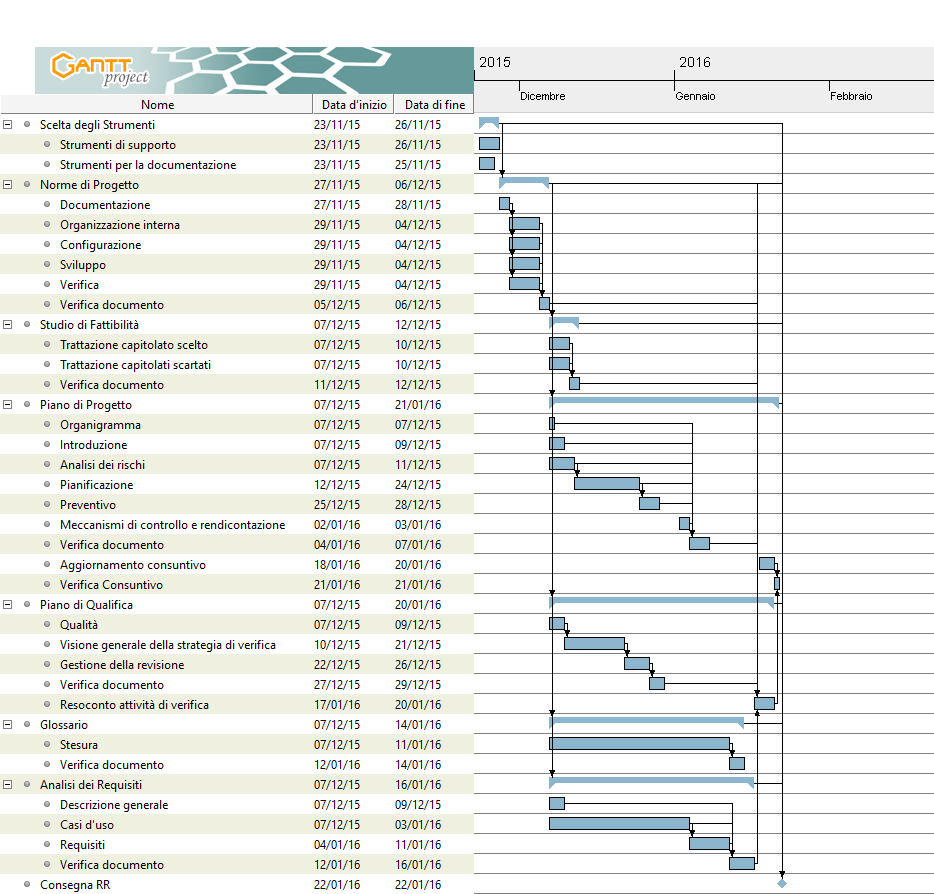
\includegraphics[width=\textwidth]{gantt_png/1-analisi}
			
		
	\subsection{Fase AD: Analisi di Dettaglio}
		\textbf{Periodo: dal 2016-02-16 al 2016-02-22}

				Questa fase comincia al termine della Fase A. È caratterizzata da una nuova analisi di tutti i documenti redatti nella fase precedente e dalla correzione in base alle richieste e segnalazioni del Committente. Gli analisti provvedono all’individuazione di nuovi requisiti, alla correzione dei requisiti segnalati e si provvede all’incremento di tutti gli altri documenti.  Aggiornati i requisiti, si terrà un incontro con il Proponente per la loro verifica.
			
		\subsubsection{Diagramma di Gantt – Fase AD}
			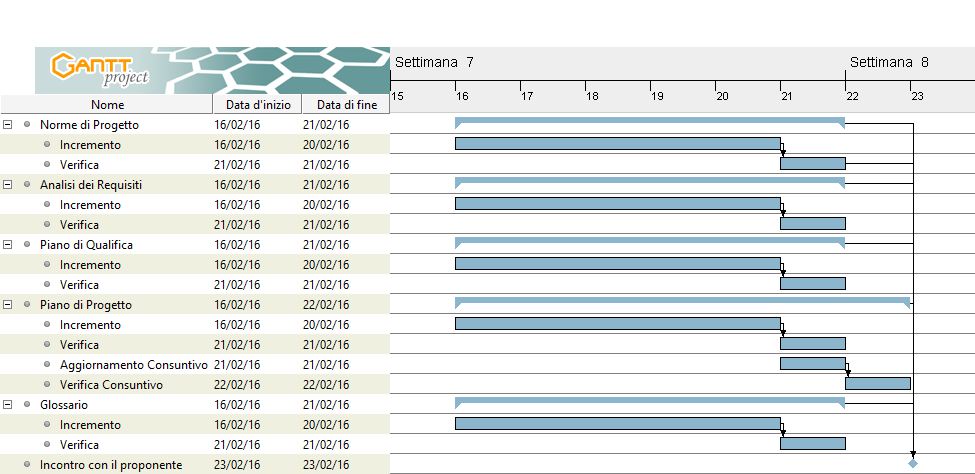
\includegraphics[width=\textwidth]{gantt_png/2-analisi_di_dettaglio}


	\end{enumerate}
\end{document}